\section{Тэхнічныя рашэнні для рэалізацыі праектаванай IP-сеткі}

\subsection{Выбар пратакола маршрутызацыі}

У якасці пратаколу маршрутызацыі можа быць абраны RIP, OSPF або якой-небудзь іншай пратакол маршрутызацыі, напрыклад IS-IS або EIGRP, у залежнасці ад тапалогіі і задач сеткі. RIP адносіцца да пратаколаў маршрутызацыі тыпу «вектар-адлегласць», тады як IS-IS і OSPF ставяцца да пратаколаў стану звяна. EIGRP з'яўляецца гібрыдным пратаколам. Разгледзім гэтыя пратаколы маршрутызацыі больш падрабязна.

\subsubsection{Пратакол OSPF.}
OSPF --- гэта адкрыты пратакол маршрутызацыі, які базіруецца на алгарытме пошуку найкарацейшага шляху (Open Shortest Path First --- OSPF). OSPF мае дзве асноўныя характарыстыкі: пратакол з'яўляецца адкрытым, г. зн. яго спецыфікацыя з'яўляецца грамадскім здабыткам, ён грунтуецца на алгарытме SPF. Алгарытм SPF часам называюць алгарытмам Дейкстры па імені яго аўтара. OSPF з'яўляецца іерархічным пратаколам маршрутызацыі з аб'яўленнем стану аб канале злучэння (link-state). Ён быў спраектаваны як пратакол работы ўнутры сеткавай вобласці --- AS (Autonomous System), якая ўяўляе сабой групу маршрутызатараў і сетак, аб'яднаных па іерархічным прынцыпе і якія знаходзяцца пад адзіным кіраваннем і сумесна выкарыстоўваюць агульную стратэгію маршрутызацыі. У якасці транспартнага пратаколу для маршрутызацыі ўнутры AS OSPF выкарыстоўвае IP-пратакол. Абмен інфармацыяй аб маршрутах ўнутры AS пратакол OSPF ажыццяўляе праз абмен паведамленнямі аб станах канала злучэнняў паміж маршрутызатарамі і сеткамі вобласці (link-state advertisement - LSA). Гэтыя паведамленні перадаюцца паміж аб'ектамі сеткі, якія знаходзяцца ў межах адной і той жа іерархічнай вобласці --- гэта можа быць як уся AS, так і некаторая група сетак ўнутры дадзенай AS. У LSA-паведамленні пратаколу OSPF ўключаецца інфармацыя аб падлучаных інтэрфейсах, пра параметры маршрутаў і іншых зменных. Па меры назапашвання маршрутызатарамі OSPF інфармацыі аб стане маршрутаў вобласці, яны разлічваюць найкарацейшы шлях да кожнага вузла, выкарыстоўваючы алгарытм SPF. Пры гэтымразлік аптымальнага маршруту ажыццяўляецца дынамічна ў адпаведнасці са зменамі тапалогіі сеткі.

Для розных тыпаў IP-сeрвісу (відаў паслуг вышэйшага ўзроўню, якія вызначаюцца значэннем поля TOS IP-пакета), OSPF можа разлічваць свае аптымальныя маршруты на падставе параметраў, найбольш крытычных для дадзенага тыпу сeрвісу. Напрыклад, якая-небудзь прыкладная праграма можа ўключыць патрабаванне аб тым, што пэўная інфармацыя з'яўляецца тэрміновай. Калі OSPF мае ў сваім распараджэнні каналы з высокім прыярытэтам, то яны могуць быць выкарыстаны для транспарціроўкі тэрміновых дэйтаграм.

OSPF падтрымлівае механізм, які дазваляе працаваць з некалькімі раўнапраўнымі маршрутамі паміж двума аб'ектамі сеткі. Гэта дазваляе істотна паменшыць час перадачы дадзеных і больш эфектыўна выкарыстоўваць каналы сувязі.

Акрамя таго, OSPF-пратакол падтрымлівае аўтэнтыфікацыю змяненняў маршрутаў. Гэта азначае, што толькі тыя маршрутызатары, якія маюць пэўныя правы, могуць ажыццяўляць маршрутызацыю пакетаў. Гэта дазваляе, пры адпаведнай настройкі правоў сістэмы маршрутызатараў, перадаваць па сетцы канфідэнцыйныя паведамленні, ведаючы загадзя, што яны праходзяць толькі па пэўных маршрутах.

Да таго ж, так як OSPF гэта пратакол стану канала, а не пратакол вектара адлегласцяў, ён мае і іншыя характарыстыкі, якія робяць яго лепш ў адносінах да RIP:
\begin{enumerate}
    \item OSPF можа разлічыць асобны набор маршрутызатараў для кожнага тыпу сeрвісу IP (type-of-service). Гэта азначае, што для любога пункта прызначэння можа быць некалькі пунктаў у табліцы маршрутызацыі, па адным для кожнага тыпу сeрвісу IP;
    \item Кожнаму інтэрфейсу прызначаецца кошт. Ён можа быць прызначаны на падставе прапускной здольнасці, часу вяртання, надзейнасці або па якому-небудзь іншаму параметру. Асобны кошт можа быць прызначаны для кожнага тыпу сeрвісу IP.
    \item Калі існуе некалькі маршрутаў да аднаго пункта прызначэння з аднолькавым коштам, OSPF размяркоўвае трафік аднольнакава паміж гэтымі маршрутамі. Гэта называецца балансіроўкай нагрузкі.
    \item Каналы пункт-пункт паміж маршрутызатарамі не маюць IP адрасоў на кожным канцы. Гэта называецца сеткамі без адраса (unnumbered). Такі падыход дазваляе зэканоміць IP адрасы.
\end{enumerate}

\subsubsection{Пратакол RIP.}
Пры выкарыстанні пратакола RIP кожны маршрутызатар рэгулярна (а таксама па асабліваму запыце па-за раскладам) рассылае сваім суседзям абвесткі, якія змяшчаюць адлегласць (вымеранае ў ліку крокаў маршрутызацыі) да ўсіх вядомых яму сетак. Сусед павялічвае адлегласць на адзін (калі казаць дакладней, то на метрыку інтэрфейсу), уносіць гэтыя маршруты ў сваю табліцу і рассылае іх усім сваім суседзям (у тым ліку і папярэдняга, але той ігнаруе іх, таму што ўжо ведае маршруты ад сябе). Максімальная даўжыня маршруту ў RIP складае 15 крокаў маршрутызацыі (hops).

Калі нейкая сетка становіцца недаступнай, то маршрутызатары працягваюць перасылаць адзін аднаму маршруты, кожны раз павялічваючы метрыку. У рэшце рэшт метрыка дасягае велічыні 16, якая азначае ў тэрмінах RIP бясконцасць, або недаступную сетку.

RIP --- самы просты з пратаколаў дынамічнай маршрутызацыі, але ён мае істотныя недахопы: марудную збежнасць, абмежаваны памер сеткі, вялікі аб'ём службовага трафіку (кожны раз рассылаецца маршрутная табліца цалкам). Апошняе робіць выкарыстанне RIP вельмі дарагім, напрыклад, у сотавых сетках. Тым не менш, RIP дагэтуль можа быць актуальны ў адносна простых і малых сетках.

\subsubsection{Пратакол IS-IS.}
IS-IS і OSPF з'яўляюцца пратаколамі стану каналаў (link state protocols), і абодва пратаколы выкарыстоўваюць алгарытм Дэйкстры для знаходжання найкарацейшага шляху. Таксама абодва пратаколы падтрымліваюць сеткавыя маскі рознай даўжыні, могуць прымяняць мультыкаставую рассылку для знаходжання найбліжэйшых маршрутызатараў, выкарыстоўваючы hello пакеты, і могуць падтрымліваць аўтэнтыфікацыю пры абнаўленні маршрутаў.

У той час як OSPF першапачаткова пабудаваны для маршрутызацыі IP адрасоў і сам працуе як пратакол 3 ўзроўню на IP, IS-IS першапачаткова з'яўляецца сеткавым узроўнем мадэлі OSI. Шырокае ўкараненне IP адрасоў спрыяла росту папулярнасці OSPF. IS-IS не выкарыстоўвае IP адрасы ў якасці маршрутаў. Ён з'яўляецца нейтральным ў дачыненні да сеткавых адрасоў, у той час OSPF быў спраектаваны для IPv4. Гэта дазваляе з лёгкасцю выкарыстоўваць IS-IS для IPv6. Для падтрымкі IPv6 сетак OSPF быў перапісаны ў OSPFv3.

Маршрутызатары IS-IS будуюць тапалагічнаe ўяўленне сеткі. Гэтая мапа паказвае падсеткі, якія IS-IS маршрутызатар можа дасягнуць, і шлях з самым нізкім коштам (найлепшы), які выкарыстоўваецца для перанакіравання трафіку.

Асноўнае адрозненне OSPF і IS-IS заключаецца ў тым як яны дзеляць аўтаномную сістэму на зоны і як ажыццяўляецца маршрутызацыя паміж зонамі. Недахоп IS-IS у тым, што маршрутызатары 2-га ўзроўню могуць мець зносіны толькі з такімі ж маршрутызатарамі, у 1-га ўзроўню --- такая ж сітуацыя. Для ўзаемадзеяння паміж маршрутызатарамі 1-га і 2-га ўзроўню і адпаведнымі зонамі выкарыстоўваюцца маршрутызатары ўзроўню 1-2. У OSPF зоны адмяжоўвацца інтэрфейсамі на маршрутызатары, такім чынам памежны маршрутызатар (area border router, ABR) можа знаходзіцца ў некалькіх зонах адначасова, эфектыўна ствараючы межы ўнутры сябе. Тады як межы IS-IS зон знаходзяцца паміж маршрутызатарамі ўзроўню 2 або ўзроўню 1-2, што робіць маршрутызатар IS-IS часткай толькі адной зоны. Таксама IS-IS не падтрымлівае нулявую зону (магістральную вобласць, праз якую можа прайсці ўвесь міжабласны трафік). Лагічным тлумачэннем гэтага з'яўляецца тое, што OSPF стварае сетку з тапалогіяй зорка з многімі зонамі перасякальнымі з нулявой, тады як IS-IS стварае лагічную тапалогію з асноўным узроўнем з маршрутызатараў 2 ўзроўню, філіялаў --- маршрутызатараў ўзроўню 1-2 і асобных абласцей з маршрутызатараў ўзроўню 1.

У пратаколе OSPF больш пашырэнняў і дадатковых функцый. Аднак пратакол IS-IS адпраўляе меншую колькасць службовага трафіку і можа маштабавацца для вялікіх сетак.

\subsubsection{Пратакол EIGRP.}
EIGRP --- удасканалены дыстанцыйна-вектарны пратакол дынамічнай маршрутызацыі, распрацаваны кампаніяй Cisco.

Дадзены пратакол маршрутызацыі папулярны ў лакальных сетках па некалькіх прычынах: настройка EIGRP даволі простая, ён устойлівы, хутка канвергуецца і для яго характэрна невысокая верагоднасць узнікнення колцавых маршрутаў. Для гэтага пратакола не трэба старанна планаваць сетку, ён просты ў канфігурацыі і пры гэтым добра маштабуецца і можа выкарыстоўвацца ў буйных сетках. Галоўны недахоп EIGRP --- закрыты стандарт. І хоць у дадзены момант кампанія Cisco адкрыла гэты пратакол, абсталяванне іншых вытворцаў можа не падтрымліваць дадзены пратакол маршрутызацыі.

Для нашай праектуемай сеткі будзем выкарыстоўваць пратакол OSPF у сувязі
з тым, што ён мае выдатныя характарыстыкі ў параўнанні з іншымі, што ён
адкрыты пратакол, а значыць пашыраецца выбар сеткавага абсталявання.
Неабходна адзначыць, што дадзены пратакол валодае высокай гібкасцю, ўлічвае асаблівасці сеткі і пры фарміраванні табліц маршрутызацыі ўлічвае прапускную здольнасць ліній, што дазваляе гібка настрайваць табліцу маршрутызацыі і тым самым паскорыць маршрутызацыю трафіку.
Адной з галоўных пераваг пратакола OSPF для праектаванай сеткі
з'яўляецца яго магчымасць настроіць асобны шлях у табліцы
маршрутызацыі для кожнага тыпу даных, гэта значыць VoIP і IPTV
трафікі будуць мець уласныя шляхі ў табліцах маршрутызацыі.

На малюнку \ref{figure: OSPF Header} прадстаўлены загаловак OSPF пакета.

\begin{figure}[h!]
    \centering
    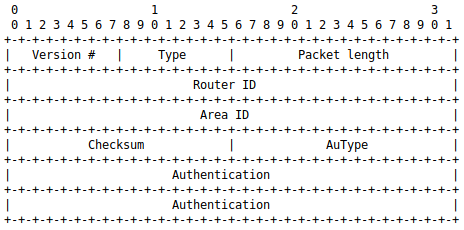
\includegraphics{ospf_header.png}
    \vspace{-0.7\baselineskip}
    \caption{Загаловак OSPF пакета}
    \label{figure: OSPF Header}
\end{figure}

Разгледзім структуру загалоўка OSPF пакета:
\begin{enumerate}
    \item Version --- версія OSPF пратакола;
    \item Type --- тып OSPF пакета:
    \begin{enumerate}
        \item Hello;
        \item Database Description;
        \item Link State Request;
        \item Link State Update;
        \item Link State Acknowledgment;
    \end{enumerate}
    \item Packet length --- даўжыня пакета ў байтах;
          уключае ў сябе стандартны OSPF загаловак;
    \item Router ID --- ідэнтыфікатара маршрутызатара крыніцы пакета;
    \item Area ID --- 32-бітны ідэнтыфікатар вобласці, да якой належыць пакет;
    \item Checksum --- кантрольная сума для праверкі змесціва пакета на памылкі;
    \item AuType --- тып аўтэнтыфікацыі:
    \begin{enumerate}
        \item 0 --- без аўтэнтыфікацыі;
        \item 1 --- пароль, які перадаецца адкрытым тэкстам;
        \item 2 --- MD5 аўтэнтыфікацыя;
    \end{enumerate}
    \item Authentication --- 64-бітнае полe для паведамлення аўтэнтыфікацыі.
\end{enumerate}



\subsection{Абаненцкі доступ да праектаванай сеткі}

У дадзеным раздзеле разгледзім некаторыя тыпы абаненцкага доступу
да праектаванай сеткі.

\subsubsection{Тэхналогія xDSL.}

DSL --- сямейства тэхналогій, якія дазваляюць значна пашырыць прапускную здольнасць абаненцкай лініі мясцовай тэлефоннай сеткі шляхам выкарыстання эфектыўных лінейных кодаў і адаптыўных метадаў карэкцыі скажэнняў лініі на аснове сучасных дасягненняў мікраэлектронікі і метадаў лічбавай апрацоўкі сігналу.

ADSL --- асіметрычная лічбавая абаненцкая лінія (Asymаetric Digital Subscriber Line) дазваляе ажыццяўляць перадачу дадзеных па асіметрычнай схеме. Дадзеная тэхналогія ператварае стандартныя тэлефонныя аналагавыя і лічбавыя лініі ў лініі высакахуткаснага доступу. Асіметрычнасць азначае, што поласы частот, якія выкарыстоўваюцца для перадачы ў розных напрамках, адрозніваюцца. Звычайна пры выкарыстанні ADSL хуткасць перадачы дадзеных па кірунку да карыстача можа быць да 8 Мбіт/с (24 Мбіт/с --- ADSL 2+), а па кірунку ад карыстальніка да 1 Мбіт/с (3,5 Мбіт/с). Хуткасць перадачы дадзеных залежыць ад працягласці абаненцкай лініі (зваротная прапарцыянальнасць). ADSL можна выкарыстоўваць для забеспячэння высакахуткаснага доступу ў сетку Інтэрнэт або, напрыклад, для перадачы відэа-патоку. Адначасова з выкарыстаннем ADSL можа выкарыстоўвацца і звычайная тэлефонная сувязь (POTS), бо для перадачы тэлефонных сігналаў не патрабуецца такая шырокая паласа частот, як для перадачы дадзеных, і дадзеныя перадаюцца ў дыяпазоне больш высокіх частот. Звычайная тэлефонная лінія выкарыстоўвае для перадачы голасу паласу частот 0 ... 4 кГц. Каб не перашкаджаць выкарыстанню тэлефоннай сеткі па яе прамым прызначэнні, у ADSL ніжняя мяжа дыяпазону частот знаходзіцца на ўзроўні 26 кГц. Верхняя ж мяжа, зыходзячы з патрабаванняў да хуткасці перадачы дадзеных і магчымасцяў тэлефоннага кабеля, складае 1,1 Мгц. Гэтая паласа прапускання дзеліцца на дзве часткі --- частоты ад 26 кГц да 138 кГц адведзены узыходзячаму патоку даных, а частоты ад 138 кГц да 1,1 МГц --- сыходным.

HDSL (High Data Rate Digital Subscriber Line) --- высакахуткасная лічбавая абаненцкая лінія. Гэта першая тэхналогія высакахуткаснай перадачы даных па скручаным медным парам тэлефонных кабеляў, якая выкарыстоўвае высокія частоты. HDSL можа апераваць хуткасцю T1 (1.544 Мбіт/с) або E1 (2 Мбіт/с). Больш нізкія хуткасці абслугоўваюцца выкарыстаннем 64 Кбіт/с каналаў, ўнутры T1/E1 пакета. З-за неабходнасці забеспячэння сіметрычнай перадачы дадзеных максімальная хуткасць падтрымліваецца толькі на адлегласці не больш за 4,5 км пры выкарыстанні адной або двух скручаных пар кабеля. Магчымая перадача дадзеных на вялікія адлегласці, пры ўмове выкарыстання рэгенератараў.

SHDSL (Single-pair High-speed Digital Subscriber Line, ITU G.991.2) --- адна з xDSL тэхналогій, якая апісвае метад перадачы сігналу па пары медных правадоў. Выкарыстоўваецца пераважна для вырашэння праблемы "апошняй мілі», г. зн. злучэнне абанентаў з вузлом доступу правайдара. Тэхналогія забяспечвае сіметрычную дуплексную перадачу даных з хуткасцямі ад 192 Kбіт/с да 2,3 Мбіт/с (з крокам у 8 Кбіт/с) па адной пары правадоў, і 4,6 Мбіт/с па двух парах.

VDSL (Very-high data rate Digital Subscriber Line) --- аналаг тэхналогіі ADSL, адрозніваецца тым, што можа працаваць як у асіметрычным, так і ў сіметрычным рэжыме. У параўнанні з ADSL VDSL мае значна больш высокую хуткасць перадачы дадзеных: ад 13 да 52 Мбіт/с у напрамку ад сеткі да карыстальніку (Downstream) і да 11 Мбіт/с ад карыстальніка да сеткі (Upstream) пры працы у асіметрычным рэжыме; максімальная прапускная здольнасць лініі VDSL пры працы ў сіметрычным рэжыме складае прыкладна 26 Мбіт/с у кожным кірунку перадачы. У залежнасці ад патрабаванай прапускной здольнасці і тыпу кабеля даўжыня лініі VDSL ляжыць у межах ад 300 метраў да 1,3 км.

\subsubsection{Тэхналогія xPON.}

Адна з найбольш папулярных аптычных тэхналогій для сетак доступу --- PON (Passive Optical Network, пасіўная аптычная сетка). Яе сутнасць у пабудове сеткі доступу, якая мае вялікую прапускную здольнасць пры мінімальных капітальных выдатках. Дадзенае рашэнне прадугледжвае стварэнне разгалінаванай, пераважна дрэвападобнай тапалогіі сеткі без актыўных кампанентаў --- на пасіўных аптычных разгаліноўшчыках. Перадача інфармацыі для ўсіх карыстальнікаў адбываецца адначасова з часовым падзелам каналаў ад галаўнога станцыі --- аптычнага лінейнага тэрмінала (Optical Line Terminal, OLT) да канцавых аптычных сеткавых блокаў (Optical Network Unit, ONU). Прыём-перадача ў абодвух напрамках, як правіла, вырабляюцца па адным аптычным валакнe, аднак на розных даўжынях хваль. Даўжыня хвалі, выкарыстоўваная ў прамым патоку (гэта значыць ад абанента да станцыі), складае 1310 нм, даўжыня хвалі ў зваротным патоку (гэта значыць ад станцыі да абанента) складае 1490 нм альбо 1550 нм. Аптычная магутнасць з выхаду OLT дзеліцца ў вузлах сеткі (раўнамерна або нераўнамерна) так, каб на ўваходзе ўсіх ONU ўзровень сігналу быў прыблізна аднолькавы. Часта адну з даўжынь хваль (у асноўным 1550 нм) вылучаюць для перадачы тэлевізійнага сігналу ўсім абанентам. На станцыі ў такім разе з мэтай аб'яднання сігналаў 1310 нм (голас, дадзеныя) і 1550 нм (відэа) усталёўваецца аптычны мультыплексар WDM. У цэлым магчыма падключыць да 32 (а ў некаторых з разнавіднасцяў --- да 64) абанентаў пры максімальнай 20-кіламетровай адлегласці сувязі.

\subsubsection{Тэхналогія WiFi.}

Тэхналогія бесправаднога доступу WiFi: Сямейства рэкамендацый 802.11 (самыя распаўсюджаныя).

Спецыяльны бесправадны інтэрфейс паміж бесправадным кліентам і базавай станцыяй або пунктам доступу, а таксама да іншых бесправадных кліентаў.

Асноўныя разнавіднасці рэкамендацыі 802.11:
\begin{enumerate}
    \item IEEE 802.11a (1997 г., 1999 г., 2001 г.):
    \begin{enumerate}
        \item хуткасць да 54 Мбіт/с, дыяпазон частот 5 Ггц;
        \item выкарыстоўвае  артаганальнаe частотнае мультыплексаванне (OFDM --- or\-tho\-go\-nal frequency division multiplexing);
    \end{enumerate}
    \item IEEE 802.11b (1999 г.):
    \begin{enumerate}
        \item хуткасць да 11 Мбіт/с (каналы на 5.5 Мбіт/с, 2 Мбіт/с і 1 Мбіт/с), дыяпазон частот 2.4 Ггц;
        \item у якасці доступу выкарыстоўвае DSSS (Direct Sequence Spread Spectrum);
    \end{enumerate}
    \item IEEE 802.11g (2003 г.):
    \begin{enumerate}
        \item ад 20 Мбіт/с, дыяпазон частот 2.4 ГГц. Аўтэнтыфікацыя па МАС-адрасах;
        \item Шыфраванне WPA 128-бітнае;
    \end{enumerate}
    \item IEEE 802.11n (2009 г.):
    \begin{enumerate}
        \item хуткасць ад 100 Мбіт/с, дыяпазон частот 2.4 Ггц;
        \item выкарыстоўвае дадатковыя метады абароны канала;
    \end{enumerate}
\end{enumerate}

\subsubsection{Тэхналогія WiMax.}

WiMAX (англ. Worldwide Interoperability for Microwave Access) --- тэлекамунікацыйная тэхналогія, распрацаваная з мэтай прадастаўлення ўніверсальнай бесправадной сувязі на вялікіх адлегласцях для шырокага спектру прылад (ад працоўных станцый і партатыўных камп'ютараў да мабільных тэлефонаў).

Заснавана на стандарце IEEE 802.16, які таксама называюць Wireless MAN
Мэта WiMAX --- падтрымка шырокапалоснага бесправаднога доступу ў сетках гарадскога маштабу (на адлегласцях некалькі дзясяткаў кіламетраў).

\subsubsection{Tэхналогія LTE.}

Адпаведна з зыходнымі данымі ў праектаванай сетцы для абаненцкага
доступу будзе выкарыстоўвацца тэхналогія LTE, таму разгледзім яе
асаблівасці і архітэктуру пабудовы падрабязней.

LTE (англ. Long-Term Evolution --- доўгачасовае развіццё) --- стандарт бесправадной высакахуткаснай перадачы даных для мабільных тэлефонаў і іншых тэрміналаў, якія працуюць з данымі. Ён заснаваны на сеткавых тэхналогіях GSM/EDGE і UMTS/HSPA, павялічваючы прапускную здольнасць і хуткасць за кошт выкарыстання іншага радыёінтэрфейса разам з паляпшэннем ядра сеткі. Стандарт быў распрацаваны 3GPP (кансорцыум, які распрацоўвае спецыфікацыі для мабільнай тэлефаніі) і вызначаны ў серыі дакументаў Release 8, з нязначнымі паляпшэннямі, апісанымі ў Release 9.

Мэтай LTE было павелічэнне прапускной здольнасці і хуткасці з выкарыстаннем новага метаду лічбавай апрацоўкі сігналаў і мадуляцыі, якія былі распрацаваны на мяжы тысячагоддзяў. Яшчэ адной мэтай было рэканструяваць і спрасціць архітэктуру сетак, заснаваных на IP, значна паменшыўшы затрымкі пры перадачы даных у параўнанні з архітэктурай 3G-сетак. Бесправадны інтэрфейс LTE з'яўляецца несумяшчальным з 2G і 3G, таму ён павінен працаваць на асобнай частаце.

Спецыфікацыя LTE дазваляе забяспечыць хуткасць загрузкі да 3 Гбіт/с, а затрымка ў перадачы даных можа быць зніжана да 2 мілісекунд. LTE падтрымлівае паласу прапускання частот ад 1,4 Мгц да 20 Мгц і падтрымлівае як частотны падзел каналаў (FDD), так і часовы падзел (TDD).

Радыус дзеяння базавай станцыі LTE залежыць ад магутнасці выпраменьвання і тэарэтычна не абмежаваны, а максімальная хуткасць перадачы даных залежыць ад радыёчастаты і аддаленасці ад базавай станцыі. Тэарэтычны мяжа для хуткасці ў 1 Гбіт/сек --- ад 3,2 км (2600 Мгц) да 19,7 км (450 Мгц). Большасць аператараў працуюць у дыяпазонах 2600 Мгц, 1800 Мгц і 800 Мгц (стандарт LTE-FDD). Базавыя станцыі дыяпазону 800 Мгц здольныя забяспечыць такую хуткасць на адлегласці да 13,4 км. Дыяпазон 1800 МГц --- найбольш выкарыстоўваецца ў свеце, ён спалучае ў сабе высокую ёмістасць і адносна вялікі радыус дзеяння (6,8 км).

Большая частка стандарту LTE разглядае мадэрнізацыю 3G UMTS на тое, што ў канчатковым выніку будзе тэхналогіяй 4G. Большая частка працы накіравана на спрашчэнне архітэктуры сістэмы: яна пераходзіць з існуючых UMTS ланцуга + камутацыі пакетаў аб'яднанай сеткі да адзінай IP-інфраструктуры (all-IP). E-UTRA з'яўляецца бесправадным інтэрфейсам LTE. Яго асноўныя асаблівасці:
\begin{enumerate}
    \item максімальная хуткасць загрузкі з Інтэрнэта да 299,6 Мбіт/с і максімальная хуткасць загрузкі ў Інтэрнэт ад абанента да 75,4 Мбіт/с у залежнасці ад катэгорыі абсталявання карыстальніка (антэна 4х4 з выкарыстаннем спектру 20 Мгц);
    \item нізкая затрымка пры перадачы дадзеных (5 мс затрымка для маленькіх IP пакетаў у аптымальных умовах), больш нізкая затрымка пры ўстаноўцы злучэння;
    \item палепшаная падтрымка мабільнасці, у якасці прыкладу тэрмінал, які рухаецца з хуткасцю 350 км/ч або 500 км/г у залежнасці ад дыяпазону частот;
    \item OFDMA для сыходнай лініі сувязі, SC-FDMA для ўзыходзячай лініі сувязі з мэтай эканоміі энергіі;
    \item падтрымка і FDD і TDD сістэм сувязі, а таксама паўдуплексных FDD з адной і той жа тэхналогіяй радыёдоступу;
    \item павышэнне гібкасці. Спектр: 1,4 Мгц, 3 МГц, 5 МГц, 10 МГц, 15 МГц і 20 МГц для шырыні соты стандартызаваны;
    \item падтрымка памераў соты ад некалькіх дзесяткаў метраў да 100 км. У ніжніх частотных дыяпазонах, якія будуць выкарыстоўвацца ў сельскіх раёнах, 5 км з'яўляецца аптымальным памерам соты. У горадзе і ў раёнах шчыльнай заселенасці больш высокія частотныя дыяпазоны (напрыклад, 2,6 Ггц) выкарыстоўваюцца для падтрымкі высакахуткаснай мабільнай шырокапалоснай сувязі. У гэтым выпадку памер соты можа быць 1 км або менш;
    \item падтрымка як мінімум 200 актыўных кліентаў у кожнай соце 5 Мгц;
    \item падтрымка суіснавання са старымі стандартамі (напрыклад, GSM/EDGE, UMTS). Карыстальнікі могуць пачаць выклік або перадачу даных у вобласці з наяўнасцю LTE і, пакінуўшы вобласць пакрыцця, працягнуць працу без якіх-небудзь адмысловых дзеянняў з яго боку ў сетках GSM/GPRS.
    \item радыёінтэрфес камутацыі пакетаў;
\end{enumerate}

На малюнкую \ref{figure: LTE structure} прадстаўлена структура
сеткі стандарту LTE.

\newpage

\begin{figure}[h!]
    \centering
    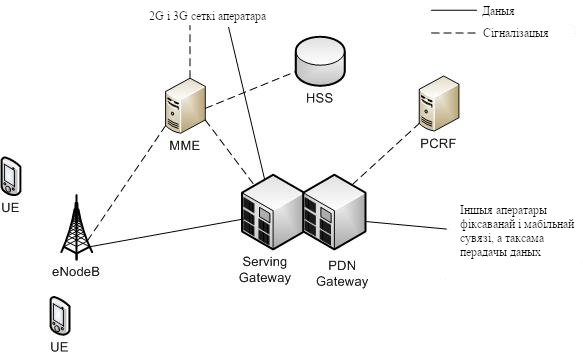
\includegraphics{lte_structure.png}
    \caption{Структура сеткі стандарту LTE}
    \label{figure: LTE structure}
\end{figure}

З малюнка \ref{figure: LTE structure} відаць, што структура сеткі моцна адрозніваецца ад сетак стандартаў 2G і 3G. Істотныя змены зведала і падсістэма базавых станцый, і падсістэма камутацыі. Была зменена тэхналогія перадачы дадых паміж абсталяваннем карыстальніка і базавай станцыяй. Таксама падвергнуліся змяненню і пратаколы перадачы даных паміж сеткавымі элементамі. Уся інфармацыя (голас, даныя) перадаецца ў выглядзе пакетаў. Такім чынам, ужо няма падзелу на часткі, якія  апрацоўваюць альбо толькі галасавую інфармацыю, альбо толькі пакетныя дадзеныя.

Можна вылучыць наступныя асноўныя элементы сеткі стандарту LTE:
\begin{enumerate}
    \item Serving SAE Gateway ці проста Serving Gateway (SGW) --- абслуговы шлюз сеткі LTE. Прызначаны для апрацоўкі і маршрутызацыі пакетных даных, якія паступаюць з/у падсістэму базавых станцый. SGW мае прамое злучэнне з сеткамі другога і трэцяга пакаленняў таго ж аператара, што спрашчае перадачу злучэння ў/з іх з прычыны пагаршэння зоны пакрыцця, перагрузак і да т. п.. У SGW няма функцыі камутацыі каналаў для галасавых злучэнняў, бо у LTE ўся інфармацыя, уключаючы голас камутуюцца і перадаецца з дапамогай пакетаў;
    \item Public Data Network SAE Gateway ці проста PDN Gateway (PGW) --- шлюз да сетак перадачы даных іншых аператараў для сеткі LTE. Асноўная задача PGW заключаецца ў маршрутызацыі трафіку сеткі LTE да іншых сетак перадачы даных, такіх як Інтэрнэт, а таксама сетак GSM, UMTS;
    \item Mobility Management Entity (MME) --- вузел кіравання мабільнасцю сеткі сотавай сувязі стандарту LTE. Прызначаны для апрацоўкі сігналізацыі, пераважна звязанай з кіраваннем мабільнасцю абанентаў у сеткі;
    \item Home Subscriber Server (HSS) --- сервер абаненцкіх даных сеткі сотавай сувязі стандарту LTE. Ўяўляе сабой вялікую базу даных і прызначаны для захоўвання даных пра абанентаў. Акрамя таго, HSS генеруе даныя, неабходныя для ажыццяўлення працэдур шыфравання, аўтэнтыфікацыі і да т. п.. Сетка LTE можа ўключаць адзін або некалькі HSS. Колькасць HSS залежыць ад геаграфічнай структуры сеткі і колькасці абанентаў;
    \item Policy and Charging Rules Function (PCRF) --- элемент сеткі сотавай сувязі стандарту LTE, які адказвае за кіраванне налічэннем платы за аказаныя паслугі сувязі, а таксама за якасць злучэнняў у адпаведнасці з заданымі канкрэтнаму абаненту характарыстыкамі.
\end{enumerate}

Для таго, каб даныя маглі быць транспартаваны праз інтэрфейс радыё LTE, выкарыстоўваюцца розныя «каналы». Яны выкарыстоўваюцца для таго, каб вылучаць розныя тыпы даных і дазволіць ім транспартавацца праз сетку доступу больш эфектыўна. Выкарыстанне некалькіх каналаў забяспечвае інтэрфейс больш высокага ўзроўню ў рамках пратаколу LTE і ўключаюць больш дакладную і пэўную сегрэгацыі даных.

Ёсць тры катэгорыі, у якія могуць быць згрупаваны розныя каналы перадачы даных:
\begin{enumerate}
    \item лагічныя каналы --- прадастаўляе паслугі сярэдняга ўзроўню кіравання доступам MAC (Medium Access Control) у межах структуры пратаколу LTE. Лагічныя каналы па тыпу перадаванай інфармацыі дзеляцца на лагічныя каналы кіравання і лагічныя каналы трафіку. Лагічныя каналы кіравання выкарыстоўваюцца для перадачы розных сігнальных і інфармацыйных паведамленняў. Па лагічным каналах трафіку перадаюць карыстальніцкія даныя;
    \item транспартныя каналы --- транспартныя каналы фізічнага ўзроўню прапануюць перадачу інфармацыі ў MAC і вышэй. Інфармацыю лагічных каналаў пасля апрацоўкі на RLC/MAC узроўнях размяшчаюць у транспартных каналах для далейшай перадачы па радыёінтэрфейсу ў фізічных каналах. Транспартны канал вызначае як і з якімі характарыстыкамі адбываецца перадача інфармацыі па радыёінтэрфейсу. Інфармацыйныя паведамленні на транспартным узроўні разбіваюць на транспартныя блокі. У кожным часавым інтэрвале перадачы (Transmission Time Interval, TTI) па радыёінтэрфейсу перадаюць хоць бы адзін транспартны блок. Пры выкарыстанні тэхналогіі MIMO магчымая перадача да чатырох блокаў у адным TTI;
    \item фізічныя каналы --- гэта каналы перадачы, якія пераносяць карыстальніцкія даныя і кіруючыя паведамленні. Яны змяняюцца паміж узыходным і сыходным патокамі, паколькі кожны з іх мае розныя патрабаванні і дзейнічае па-свойму.
\end{enumerate}

Для праектаванай сеткі будуць выкарыстоўвацца LTE, для мабільнай сувязі, і
GPON, для фіксаванай сувязі, тэхналогіі абаненцкага доступу.
Былі абраныя дадзеныя тэхналогіі абаненцкага доступу ў сувязі з тым,
што яны з'яўляюцца найбольш перспектыўнымі і распаўсюджанымі, у выпадку з GPON, у Беларусі, што дазваляе пашырыць абхват тэрыторыі, на якой
падключаюцца абаненты.

Кожная з гэтых тэхналогій абаненцкага доступу прадастаўляе шырокія
магчымасці, такія як прапускная здольнасць і прастата падключэння
абанентаў да сеткі правайдара.

\subsection{Выбар сеткавага абсталявання}

Неабходна ажыццявіць выбар абсталявання, якое патрабуецца для пабудовы сеткі, г.зн. трэба выбраць маршрутызатары, шлюз VoIP, сервер IPTV.

Для выбару абсталявання неабходна ўлічваць наступныя патрабаванні. Шлюз VoIP павінен падтрымліваць пратакол, які забяспечвае зададзеную ў праекце хуткасць кадавання прамовы (16 кбіт/с). У складзе IPTV-сервера павінен быць кодэк MPEG-4 зададзенай у праекце хуткасцю (24 Мбіт/с), а маршрутызатары павінны падтрымліваць абраны пратакол маршрутызацыі (OSPF) і мець прадукцыйнасць не менш значэння разлічанай інтэнсіўнасці нагрузкі.

У якасці VoIP шлюза быў абраны SNR-VG-6040. Дадзены шлюз падтрымлівае
пратакол G.726 з хуткасцю кадавання мовы 16 Кбіт/с, што адпавядае
заданню праекта.

VoIP шлюз SNR --- высокатэхналагічнае і надзейнае рашэнне для сетак IP-тэлефаніі. Спалучаючы ў сабе высокую якасць перадачы голасу, багаты функцыянал, а таксама кампактныя памеры і нізкі кошт, VoIP шлюзы SNR-VG з'яўляюцца аптымальным выбарам для інтэграцыі IP-тэлефаніі. Сумяшчальнасць з рознымі правайдарамі VoIP, а таксама IP-PBX і праграмнымі камутатарамі розных вытворцаў робіць галасавыя шлюзы SNR-VG універсальным рашэннем, цалкам адпаведным сучасным патрабаванням да прылад IP тэлефаніі.

VoIP шлюзы серыі SNR-VG-6000 адрозніваюцца прастатой і інтуітыўнасцю ў настройцы. Прыемны інтэрфейс, галасавое меню для канфігурацыі робяць шлюзы IP тэлефаніі серыі SNR-VG-6000 даступным і прывабным рашэннем для розных груп карыстальнікаў.

Шлюзы IP тэлефаніі SNR-VG валодаюць усім неабходным функцыяналам, запатрабаваным на сённяшні дзень сярод карыстальнікаў IP-тэлефаніі. Прылады падтрымліваюць функцыянал Fax-over-IP (T.38, G.711 pass-through), могуць працаваць у рэжымах Router/Bridge, падтрымліваюць NAT.

SNR-VG-6040 --- шлюз для IP тэлефаніі стандарту SIP, які аб'ядноўвае ў сабе перадачу даных і галасу, перадачу факса. Прылада ідэальна інтэгруецца ў любыя сеткі, дазваляе эфектыўна аб'ядноўваць сеткавую інфраструктуру прадпрыемства з лініямі ТфАK. Мае 4 парты FXO і 2 парты Ethernet.

Характарыстыкі дадзенага шлюза прыведзеныя ў табліцы
\ref{table: SNR-VG-6040}.

У якасці сервера IPTV абярэм Cisco IPTV 3400, які ўяўляе
сабой камбінацыю ўнікальнага праграмнага забеспячэння, прызначанага для
арганізацыі перадачы і прыёму высакаякаснага відэа на неабмежаваную колькасць камп'ютараў па IP-сетцы.

Серверы Cisco IPTV 3400 існуюць як у выглядзе праграмнага забеспячэння, так і ў
выглядзе спецыялізаванага апаратна-праграмнага комплексу прадуктаў серыі Cicso IPTV 3400, у склад якога ўваходзяць наступныя прылады:
\begin{enumerate}
    \item сервер-кіраўнік Cicso IPTV 3412 Control Server;
    \item шырокавяшчальны сервер Cisco IPTV 3425 Broadcast Servers;
    \item архіўны сервер Cisco IPT 3432 Archive Server;
    \item стартавая відэасістэма Cisco IPTV 3417 Video Starter System;
    \item кліенцкае ПЗ Cisco IPTV Viewer;
\end{enumerate}

Асноўныя магчымасці дадзена IPTV сервера:
\begin{enumerate}
    \item Для зручнасці карыстальнікаў сістэма Cisco IPTV падтрымлівае тры рэжыму перадачы відэа: прамую, запланаваную трансляцыю і трансляцыю па патрабаванні;
    \item Сістэма Cisco IPTV падтрымлівае інтэрактыўны доступ у Інтэрнэт праз web-інтэрфейс, а таксама дазваляе арганізаваць зваротную сувязь з карыстальнікамі;
    \item Дзякуючы ўжыванню тэхналогіі IP Multicast сістэма Cisco IPTV валодае найвышэйшай маштабаванасцю і дазваляе арганізоўваць трансляцыю як для некалькіх, так і для некалькіх тысяч карыстальнікаў, выкарыстоўваючы мінімальную паласу прапускання;
    \item Сістэма Cisco IPTV выкарыстоўвае стандарты RTP/RTCP для перадачы відэа ў рэжыме рэальнага часу, відэакодэкі Vxtreme, H.261, MPEG-1, MPEG-2, MPEG-4, Indeo 4.1, Apple QuickTime;
    \item Падтрымка фарматаў ASF, AVI, MP3 і MPEG.
\end{enumerate}

Дадзены сервер адпавядае зададзеным патрабаванням (падтрымка MPEG-4).
Тэхнічная характарыстыка прыведзеная ў табліцы
\ref{table: Cisco IPTV 3427-C1}.

У якасці маршрутызатараў на праектаванай сеткі абярэм Huawei NE40E. Серыя універсальных паслуговых маршрутызатараў NetEngine40E (NE40E) --- сямейства сеткавага абсталявання класа high-end. Яны звычайна ўжываюцца на межах магістральных сетак пратаколу IP, гарадскіх IP-сетак (MAN), і іншых маштабных IP-сетак. Маршрутызатары NE40E ўяўляюць сабой закончаны шматузроўневае рашэнне для IP-сетак.

NE40E забяспечвае функцыі MSE (Multi Service Edge) для кантролю доступу і кіравання карыстальнікаў DHCP, IP over Ethernet (IPoE) і вылучаных ліній. MSE забяспечвае дынамічны карыстальніцкі доступ кіравання карыстальнікамі,
карыстальніцкую аўтэнтыфікацыю і ўлік, а таксама планаванне QoS. Акрамя таго, MSE рэалізуе функцыю прадастаўленне паласы па патрабаванню BoD (Bandwidth on Demand) для карпаратыўных паслуг і асобных карыстальнікаў DHCP.

NE40E падтрымлівае разнастайныя функцыі IPv6, уключаючы вылучаную лінію IPv6, двайны стэк, тэхналогіі тунэлявання і пераўтварэнні сеткавых адрасоў. Прылады NE40E падтрымліваюць тэхналогію Next Hop Separation, якая дазваляе скараціць час пераўтварэння IPv6, а таксама табліцу маршрутызацыі IPv6 FIB большага аб'ёму, якая дазваляе пашырыць магчымасці маштабавання. Названыя тэхналогіі дазваляюць ствараць розныя высокапрадукцыйныя рашэнні для пераходу з IPv4 на IPv6.

Тэхнічныя характарыстыкі абранага абсталявання прыведзены ў
табліцы \ref{table: NE40E}.

Такім чынам, абрана сеткавае абсталяванне, якое ў поўнай меры здольна задаволіць зададзеныя сеткавыя патрабаванні.
